% ============================================================
%  INFORME TÉCNICO — SIMULACIÓN DES PANADERÍA SUPERMERCADO
%  Capstone Analytics · Universidad del Desarrollo · Mayo 2026
% ============================================================
\documentclass[10pt, a4paper]{article}

% --- Codificación y lenguaje ---
\usepackage[utf8]{inputenc}
\usepackage[T1]{fontenc}
% babel-spanish no disponible; se omite opción de idioma
\usepackage{babel}

% --- Tipografía ---
\usepackage{lmodern}
\usepackage{microtype}

% --- Geometría y márgenes ---
\usepackage[
  top=2.5cm, bottom=2.5cm,
  left=2.8cm, right=2.8cm,
  headheight=15pt
]{geometry}
\usepackage{pdflscape}   % páginas en orientación landscape para figuras anchas

% --- Encabezado y pie de página ---
\usepackage{fancyhdr}
\pagestyle{fancy}
\fancyhf{}
\fancyhead[L]{\small\textit{Informe T\'ecnico --- Panader\'ia Supermercado}}
\fancyhead[R]{\small\textit{Capstone Analytics $\cdot$ UDD}}
\fancyfoot[C]{\thepage}
\renewcommand{\headrulewidth}{0.4pt}

% --- Colores y gráficos ---
\usepackage[dvipsnames,table]{xcolor}
\usepackage{graphicx}
\usepackage{tikz}
\usetikzlibrary{shapes.geometric, arrows.meta, positioning, fit, backgrounds,
                decorations.pathreplacing, calc, matrix}
\usepackage{pgfplots}
\pgfplotsset{compat=1.18}

% --- Tablas profesionales ---
\usepackage{booktabs}
\usepackage{multirow}
\usepackage{makecell}
\usepackage{array}
\usepackage{longtable}
\usepackage{tabularx}
\usepackage{colortbl}

% --- Listas y enumeraciones ---
\usepackage{enumitem}
\setlist[itemize]{leftmargin=1.5em, topsep=3pt, itemsep=2pt}
\setlist[enumerate]{leftmargin=1.5em, topsep=3pt, itemsep=2pt}

% --- Matemáticas ---
\usepackage{amsmath, amssymb}

% --- Flotantes y captions ---
\usepackage{float}
\usepackage{caption}
\captionsetup{
  font=small, labelfont=bf,
  format=hang, margin=10pt,
  skip=6pt
}
\usepackage{subcaption}

% --- Hiperlinks (debe ir al final) ---
\usepackage[
  colorlinks=true,
  linkcolor=NavyBlue,
  citecolor=NavyBlue,
  urlcolor=NavyBlue
]{hyperref}

% --- Paleta de colores corporativa ---
\definecolor{azulUDD}{RGB}{0,61,121}
\definecolor{azulClaro}{RGB}{210,228,246}
\definecolor{rojoAlerta}{RGB}{192,0,0}
\definecolor{verdeOK}{RGB}{0,128,0}
\definecolor{grisClaro}{RGB}{245,245,245}
\definecolor{naranjaAccento}{RGB}{220,100,0}

% --- Estilos compartidos para flowcharts (diseño plano) ---
\tikzset{
  fc/start/.style={rectangle, draw=azulUDD, fill=white,
    minimum width=32mm, minimum height=9mm,
    font=\scriptsize\bfseries\color{azulUDD}, align=center, line width=1pt},
  fc/end/.style={rectangle, draw=azulUDD, fill=white,
    minimum width=32mm, minimum height=9mm,
    font=\scriptsize\bfseries\color{azulUDD}, align=center, line width=1pt,
    double, double distance=1pt},
  fc/op/.style={rectangle, draw=azulUDD, fill=white,
    minimum width=46mm, minimum height=10mm,
    font=\scriptsize\color{black}, align=center, line width=0.6pt,
    text width=44mm, inner sep=2pt},
  fc/op2/.style={rectangle, draw=azulUDD, fill=azulUDD!6,
    minimum width=46mm, minimum height=10mm,
    font=\scriptsize\color{black}, align=center, line width=0.6pt,
    text width=44mm, inner sep=2pt},
  fc/dec/.style={diamond, draw=naranjaAccento, fill=white,
    aspect=2.2, inner sep=1pt, font=\tiny\color{black}, align=center,
    line width=0.8pt, text width=36mm},
  fc/arr/.style={-{Stealth[length=4pt,width=4pt]}, line width=0.6pt,
    draw=azulUDD},
  fc/lbl/.style={font=\tiny\itshape\color{azulUDD!80!black},
    fill=white, inner sep=1pt}
}

% ============================================================
%  PORTADA
% ============================================================
\begin{document}

\begin{titlepage}
  \centering
  \vspace*{1.5cm}

  {\color{azulUDD}\rule{\linewidth}{1.5pt}}
  \vspace{0.4cm}

  {\LARGE\bfseries\color{azulUDD}
    Redise\~no Operacional de la Panader\'ia:\\[6pt]
    D\'onde Invertir y D\'onde No
  }

  \vspace{0.3cm}
  {\color{azulUDD}\rule{\linewidth}{0.8pt}}
  \vspace{0.6cm}

  {\large\itshape Informe T\'ecnico de Simulaci\'on --- Proyecto Capstone Analytics}

  \vspace{1.2cm}

  {\normalsize
    \begin{tabular}{ll}
      \textbf{Instituci\'on:}       & Universidad del Desarrollo \\[4pt]
      \textbf{Asignatura:}          & Capstone Simulaci\'on \\[4pt]
      \textbf{Fecha:}               & Mayo 2026 \\[4pt]
      \textbf{Confidencialidad:}    & Uso interno --- Gerencia de Operaciones \\
    \end{tabular}
  }

  \vspace{2cm}

  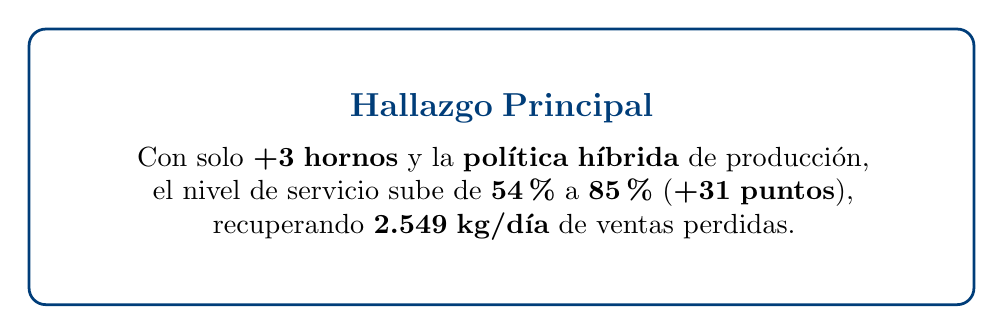
\begin{tikzpicture}
    \draw[azulUDD, line width=1pt, rounded corners=6pt]
      (0,0) rectangle (12,3.5);
    \node[align=center, text width=11cm] at (6,1.75) {
      {\large\bfseries\color{azulUDD} Hallazgo Principal}\\[6pt]
      {\normalsize
        Con solo \textbf{+3 hornos} y la \textbf{pol\'itica h\'ibrida} de producci\'on,\\
        el nivel de servicio sube de \textbf{54\,\%} a \textbf{85\,\%} (\textbf{+31 puntos}),\\
        recuperando \textbf{2.549 kg/d\'ia} de ventas perdidas.}
    };
  \end{tikzpicture}

  \vfill

  {\color{azulUDD}\rule{\linewidth}{1.5pt}}
  {\small \textit{Elaborado mediante Simulaci\'on de Eventos Discretos en SIMIO
    $\cdot$ 650 corridas $\cdot$ 13 escenarios $\times$ 50 r\'eplicas}}
\end{titlepage}

% ============================================================
%  TABLA DE CONTENIDOS
% ============================================================
\tableofcontents
\newpage

% ============================================================
%  1. RESUMEN EJECUTIVO
% ============================================================
\section{Resumen Ejecutivo}
\label{sec:resumen}

% TODO: redactar al final

\newpage

% ============================================================
%  2. DESCRIPCIÓN DEL SISTEMA
% ============================================================
\section{Descripci\'on del Sistema}
\label{sec:sistema}

\subsection{Operaci\'on General}

La panader\'ia opera como una unidad productiva integrada dentro del
supermercado, dedicada exclusivamente a abastecer una zona de autoservicio con
pan fresco durante la ventana comercial de 09:00 a 21:00. La operaci\'on
se estructura en tres subsistemas interdependientes: (i) una l\'inea
productiva que transforma materias primas en lotes de pan listo para horneado,
(ii) una gesti\'on de hornos que agrupa, hornea y enfr\'ia los lotes por
familias de cocci\'on, y (iii) una sala de ventas que mantiene un
inventario por tipo de pan expuesto al consumo estoc\'astico de los clientes.

Para garantizar disponibilidad inicial al momento de la apertura, la producci\'on
se inicia a las 06:00 ---tres horas antes que la tienda--- y se
mantiene continua durante toda la jornada. La demanda total a atender asciende
a 8.200\,kg/d\'ia distribuidos entre los 10 productos del portafolio.
Una caracter\'istica cr\'itica del negocio es que no existe sustituci\'on
entre productos: si un cliente busca un tipo espec\'ifico de pan y este no se
encuentra disponible en g\'ondola, la venta se pierde sin posibilidad de
recuperaci\'on. Esto convierte cada quiebre de stock en una venta perdida
contabilizable y motiva el dise\~no centrado en minimizar dichos eventos.

\subsection{Portafolio de Productos}

La panader\'ia elabora 10 tipos de pan agrupados en tres familias de horneado
seg\'un su tiempo de cocci\'on. Esta clasificaci\'on no es arbitraria: define
la restricci\'on operacional m\'as importante del sistema, dado que los hornos
solo pueden procesar productos de una misma familia por corrida y requieren un
tiempo de \textit{setup} al cambiar entre ellas. La Tabla~\ref{tab:productos}
consolida el portafolio, ordenado por familia y demanda diaria.

\begin{table}[H]
\centering
\caption{Portafolio de productos, familias de horneado y participaci\'on de demanda.}
\label{tab:productos}
\renewcommand{\arraystretch}{1.30}
\setlength{\tabcolsep}{6pt}
\begin{tabular}{c l c r r c}
\toprule
\rowcolor{azulClaro}
\textbf{\#} & \textbf{Tipo de Pan} & \textbf{Familia} & \textbf{Demanda} & \textbf{\%} & \textbf{T.\ Horn.} \\
\rowcolor{azulClaro}
            &                     &                  & \textbf{(kg/d\'ia)} &             &                       \\
\midrule
\multicolumn{6}{l}{\cellcolor{azulUDD!10}\textbf{Familia 1 --- Horneado corto (14 min)}} \\
5 & Pan Hot Dog       & F1 & 1.200 & 14{,}6\,\% & 14 min \\
\rowcolor{grisClaro}
8 & Dobladita         & F1 & 350   & 4{,}3\,\%  & 14 min \\
9 & Bocado de Dama    & F1 & 220   & 2{,}7\,\%  & 14 min \\
\midrule
\multicolumn{6}{l}{\cellcolor{azulUDD!10}\textbf{Familia 2 --- Horneado medio (18 min)}} \\
\rowcolor{grisClaro}
1  & Marraqueta         & F2 & 2.000 & 24{,}4\,\% & 18 min \\
2  & Hallulla           & F2 & 1.700 & 20{,}7\,\% & 18 min \\
\rowcolor{grisClaro}
4  & Hallulla Integral  & F2 & 800   & 9{,}8\,\%  & 18 min \\
10 & Amasado            & F2 & 380   & 4{,}6\,\%  & 18 min \\
\midrule
\multicolumn{6}{l}{\cellcolor{azulUDD!10}\textbf{Familia 3 --- Horneado largo (21 min)}} \\
\rowcolor{grisClaro}
3 & Marraqueta Integral & F3 & 800   & 9{,}8\,\%  & 21 min \\
6 & Ciabatta            & F3 & 400   & 4{,}9\,\%  & 21 min \\
\rowcolor{grisClaro}
7 & Baguette            & F3 & 350   & 4{,}3\,\%  & 21 min \\
\midrule
\rowcolor{azulClaro}
\multicolumn{3}{r}{\textbf{TOTAL}} & \textbf{8.200} & \textbf{100\,\%} & --- \\
\bottomrule
\end{tabular}
\end{table}

Dos observaciones clave emergen del portafolio: primero, la demanda se concentra
fuertemente en Marraqueta y Hallulla (45{,}1\,\% combinado, ambos de la
Familia~2), de modo que la capacidad de horneado en esta familia define en gran
parte el rendimiento del sistema; segundo, la Familia~3 (Marraqueta Integral,
Ciabatta y Baguette) tiene el ciclo de cocci\'on m\'as largo (21 min) pero
volumen relativamente bajo (19{,}0\,\%), lo que la convierte en candidata
natural para corridas de cierre de jornada.

\subsection{Flujo Productivo de Alto Nivel}

Cada lote de pan recorre nueve etapas secuenciales antes de llegar a
g\'ondola, distribuidas entre los tres subsistemas descritos en
\S\ref{sec:sistema}.1. La Figura~\ref{fig:bpmn} presenta el flujo completo
modelado bajo la notaci\'on BPMN\,2.0, organizado en tres calles (\emph{lanes})
que reflejan las responsabilidades operativas: producci\'on, gesti\'on de hornos
y sala de ventas.

% =====================================================================
%  DIAGRAMA BPMN — Tres lanes alineados con coordenadas absolutas
% =====================================================================
\begin{landscape}
\begin{figure}[H]
\centering
\resizebox{0.95\linewidth}{!}{%
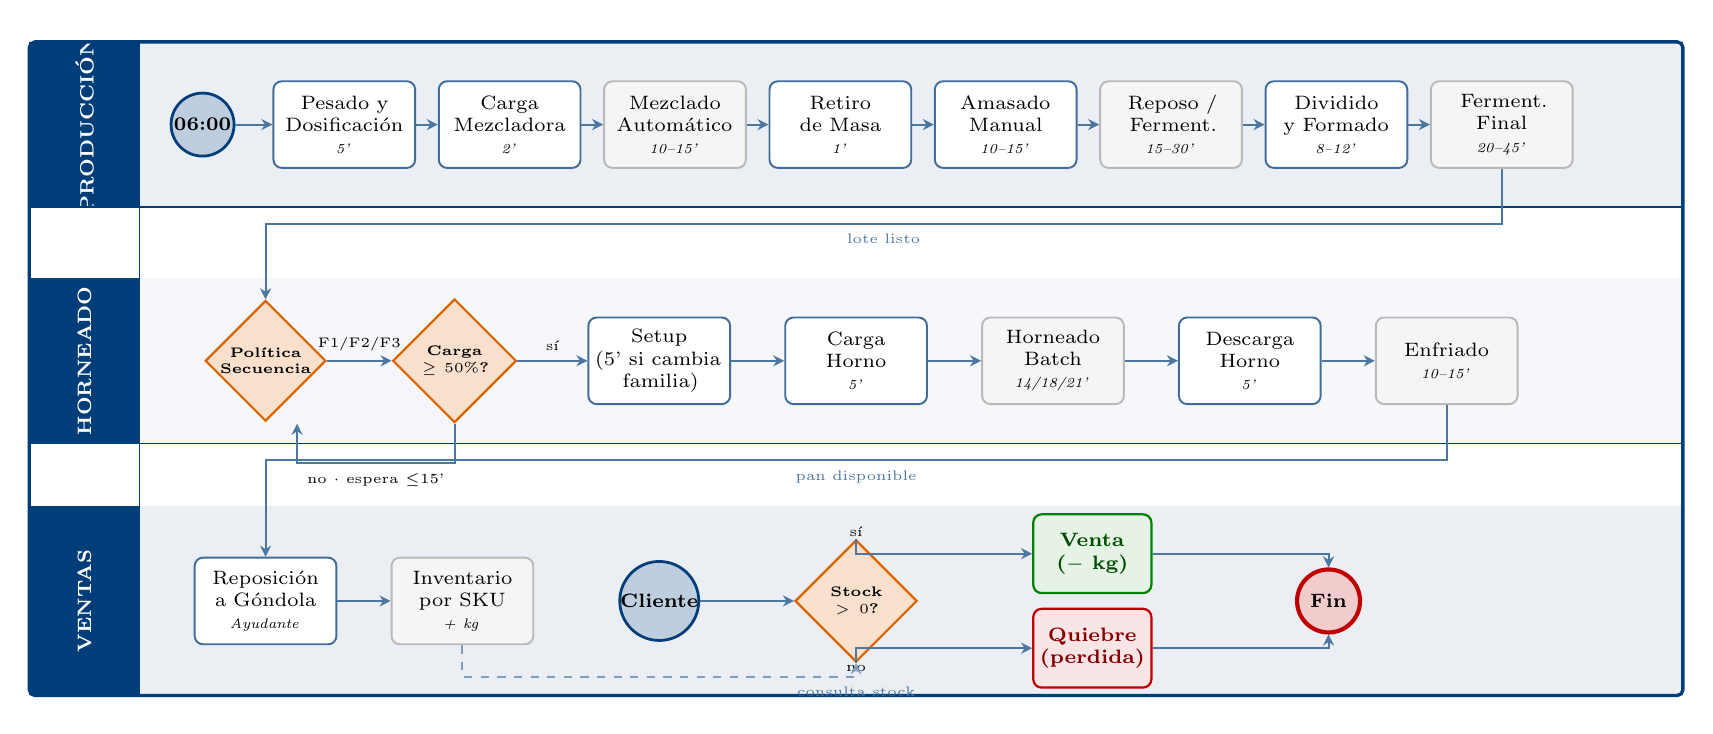
\begin{tikzpicture}[
  x=1cm, y=1cm,
  % --- Estilos ---
  startevent/.style={
    circle, draw=azulUDD, fill=azulUDD!25,
    minimum size=8mm, line width=1pt,
    font=\scriptsize\bfseries, align=center, inner sep=0pt},
  endevent/.style={
    circle, draw=rojoAlerta, fill=rojoAlerta!20,
    minimum size=8mm, line width=1.5pt,
    font=\scriptsize\bfseries, align=center, inner sep=0pt},
  task/.style={
    rectangle, rounded corners=3pt,
    draw=azulUDD!75, fill=white, line width=0.7pt,
    minimum width=18mm, minimum height=11mm,
    font=\scriptsize, align=center, text width=17mm, inner sep=1pt},
  taskauto/.style={
    rectangle, rounded corners=3pt,
    draw=gray!55, fill=grisClaro, line width=0.7pt,
    minimum width=18mm, minimum height=11mm,
    font=\scriptsize, align=center, text width=17mm, inner sep=1pt},
  taskout/.style={
    rectangle, rounded corners=3pt,
    draw=verdeOK, fill=verdeOK!10, line width=0.8pt,
    minimum width=15mm, minimum height=10mm,
    font=\scriptsize\bfseries, align=center, text width=14mm, inner sep=1pt,
    text=verdeOK!60!black},
  taskbad/.style={
    rectangle, rounded corners=3pt,
    draw=rojoAlerta, fill=rojoAlerta!10, line width=0.8pt,
    minimum width=15mm, minimum height=10mm,
    font=\scriptsize\bfseries, align=center, text width=14mm, inner sep=1pt,
    text=rojoAlerta!70!black},
  gw/.style={
    diamond, draw=naranjaAccento, fill=naranjaAccento!20,
    minimum size=8mm, inner sep=0pt,
    font=\tiny\bfseries, align=center, line width=0.8pt,
    text width=12mm},
  arrow/.style={
    -{Stealth[length=4pt,width=4pt]},
    line width=0.7pt, draw=azulUDD!70},
  msgarrow/.style={
    -{Stealth[length=4pt,width=4pt]},
    line width=0.8pt, draw=naranjaAccento, dashed},
  lanelabel/.style={
    rectangle, fill=azulUDD, text=white,
    font=\footnotesize\bfseries, align=center,
    rotate=90, minimum width=18mm, minimum height=6mm,
    inner sep=2pt},
  laneband/.style={
    rectangle, fill=azulUDD!8, line width=0pt,
    inner sep=0pt}
]

% =====================================================================
%  FONDOS DE LANES (calles del pool)
% =====================================================================
% Contenido de las calles (fondo claro)
\fill[azulUDD!8]  (1.4, 6.5) rectangle (21.0, 8.6);   % Lane 1 content
\fill[azulUDD!4]  (1.4, 3.5) rectangle (21.0, 5.6);   % Lane 2 content
\fill[azulUDD!8]  (1.4, 0.3) rectangle (21.0, 2.7);   % Lane 3 content

% Franja izquierda de cada calle (etiqueta de rol)
\fill[azulUDD]    (0.0, 6.5) rectangle (1.4, 8.6);   % Lane 1 label strip
\fill[azulUDD]    (0.0, 3.5) rectangle (1.4, 5.6);   % Lane 2 label strip
\fill[azulUDD]    (0.0, 0.3) rectangle (1.4, 2.7);   % Lane 3 label strip

% Lane labels (texto rotado dentro de cada franja)
\node[white, font=\scriptsize\bfseries, rotate=90] at (0.7, 7.55) {PRODUCCI\'ON};
\node[white, font=\scriptsize\bfseries, rotate=90] at (0.7, 4.55) {HORNEADO};
\node[white, font=\scriptsize\bfseries, rotate=90] at (0.7, 1.50) {VENTAS};

% Pool exterior (contorno)
\draw[azulUDD, line width=1.2pt, rounded corners=2pt]
  (0.0, 0.3) rectangle (21.0, 8.6);

% Separadores entre lanes
\draw[azulUDD, line width=0.6pt] (0, 6.5) -- (21.0, 6.5);
\draw[azulUDD, line width=0.6pt] (0, 3.5) -- (21.0, 3.5);

% Separador entre franja de etiqueta y contenido
\draw[azulUDD, line width=0.6pt] (1.4, 0.3) -- (1.4, 8.6);

% =====================================================================
%  LANE 1 — PRODUCCIÓN  (tasks at y=7.55)
% =====================================================================
\node[startevent] at (2.2,  7.55) (start)   {06:00};
\node[task]       at (4.0,  7.55) (pesado)  {Pesado y\\Dosificaci\'on\\{\tiny\textit{5'}}};
\node[task]       at (6.1,  7.55) (cmez)    {Carga\\Mezcladora\\{\tiny\textit{2'}}};
\node[taskauto]   at (8.2,  7.55) (mezcla)  {Mezclado\\Autom\'atico\\{\tiny\textit{10--15'}}};
\node[task]       at (10.3, 7.55) (retiro)  {Retiro\\de Masa\\{\tiny\textit{1'}}};
\node[task]       at (12.4, 7.55) (amasado) {Amasado\\Manual\\{\tiny\textit{10--15'}}};
\node[taskauto]   at (14.5, 7.55) (reposo)  {Reposo /\\Ferment.\\{\tiny\textit{15--30'}}};
\node[task]       at (16.6, 7.55) (formado) {Dividido\\y Formado\\{\tiny\textit{8--12'}}};
\node[taskauto]   at (18.7, 7.55) (ferm2)   {Ferment.\\Final\\{\tiny\textit{20--45'}}};

\draw[arrow] (start)  -- (pesado);
\draw[arrow] (pesado) -- (cmez);
\draw[arrow] (cmez)   -- (mezcla);
\draw[arrow] (mezcla) -- (retiro);
\draw[arrow] (retiro) -- (amasado);
\draw[arrow] (amasado)-- (reposo);
\draw[arrow] (reposo) -- (formado);
\draw[arrow] (formado)-- (ferm2);

% =====================================================================
%  LANE 2 — GESTIÓN DE HORNOS  (tasks at y=4.55)
% =====================================================================
\node[gw]         at (3.0,  4.55) (gwseq)   {Pol\'itica\\Secuencia};
\node[gw]         at (5.4,  4.55) (gwcarga) {Carga\\$\geq50\%$?};
\node[task]       at (8.0,  4.55) (setup)   {Setup\\(5' si cambia\\familia)};
\node[task]       at (10.5, 4.55) (cargah)  {Carga\\Horno\\{\tiny\textit{5'}}};
\node[taskauto]   at (13.0, 4.55) (hornead) {Horneado\\Batch\\{\tiny\textit{14/18/21'}}};
\node[task]       at (15.5, 4.55) (descarga){Descarga\\Horno\\{\tiny\textit{5'}}};
\node[taskauto]   at (18.0, 4.55) (enfriado){Enfriado\\{\tiny\textit{10--15'}}};

\draw[arrow] (gwseq)    -- node[above, font=\tiny]{F1/F2/F3} (gwcarga);
\draw[arrow] (gwcarga)  -- node[above, font=\tiny]{s\'i} (setup);
\draw[arrow] (setup)    -- (cargah);
\draw[arrow] (cargah)   -- (hornead);
\draw[arrow] (hornead)  -- (descarga);
\draw[arrow] (descarga) -- (enfriado);

% Loop de espera por carga insuficiente
\draw[arrow] (gwcarga.south) -- ++(0,-0.5)
  -- node[below, font=\tiny]{no $\cdot$ espera $\leq$15'} ++(-2.0,0)
  -- ++(0,0.5);

% =====================================================================
%  LANE 3 — SALA DE VENTAS  (tasks at y=1.50)
% =====================================================================
\node[task]      at (3.0,  1.50) (repo)    {Reposici\'on\\a G\'ondola\\{\tiny\textit{Ayudante}}};
\node[taskauto]  at (5.5,  1.50) (inv)     {Inventario\\por SKU\\{\tiny\textit{+ kg}}};
\node[startevent]at (8.0,  1.50) (cli)     {Cliente};
\node[gw]        at (10.5, 1.50) (gwstk)   {Stock\\$>0$?};
\node[taskout]   at (13.5, 2.10) (venta)   {Venta\\($-$ kg)};
\node[taskbad]   at (13.5, 0.90) (quiebre) {Quiebre\\(perdida)};
\node[endevent]  at (16.5, 1.50) (fin)     {Fin};

\draw[arrow] (repo)  -- (inv);
\draw[arrow] (cli)   -- (gwstk);
\draw[arrow] (gwstk.north) |- (venta.west)   node[pos=0.25, above, font=\tiny]{s\'i};
\draw[arrow] (gwstk.south) |- (quiebre.west) node[pos=0.25, below, font=\tiny]{no};
\draw[arrow] (venta.east)   -| (fin.north);
\draw[arrow] (quiebre.east) -| (fin.south);

% El inventario alimenta al gateway de stock (lectura) — ruta inferior
\draw[arrow, dashed, draw=azulUDD!50]
  (inv.south) -- ++(0,-0.4) -| (gwstk.south)
  node[pos=0.5, below, font=\tiny\color{azulUDD!70}]{consulta stock};

% =====================================================================
%  FLUJOS ENTRE LANES (sequence flow cruzando calles)
% =====================================================================
% Producción → Horneado : ferm2 -> gwseq
\draw[arrow] (ferm2.south) -- ++(0,-0.7)
  -| (gwseq.north)
  node[pos=0.25, below, font=\tiny\color{azulUDD!70}]{lote listo};

% Horneado → Sala : enfriado -> repo
\draw[arrow] (enfriado.south) -- ++(0,-0.7)
  -| (repo.north)
  node[pos=0.25, below, font=\tiny\color{azulUDD!70}]{pan disponible};

\end{tikzpicture}%
}
\caption{Diagrama BPMN\,2.0 del sistema panader\'ia supermercado. Las cajas con
fondo blanco indican actividades con intervenci\'on de recurso humano; las cajas
en gris representan procesos autom\'aticos o sin intervenci\'on. Los diamantes
naranjas son \emph{gateways} (decisiones). La l\'inea punteada naranja
representa el flujo de retroalimentaci\'on (se\~nal de stock bajo) que informa
la pol\'itica de secuencia de producci\'on.}
\label{fig:bpmn}
\end{figure}
\end{landscape}

El proceso encadena tareas con distintas naturalezas: actividades manuales
---realizadas por el panadero (pesado, carga/retiro de mezcladora, amasado,
formado)---, actividades autom\'aticas ---realizadas por la maquinaria sin
intervenci\'on humana (ciclo de mezclado, reposo, fermentaci\'on, horneado,
enfriado)---, y actividades de operaci\'on de hornos ---ejecutadas por
manipuladores (carga, descarga). El detalle granular de tiempos por etapa y
por tipo de pan, base para los c\'alculos de capacidad, se documenta en el
Anexo~\ref{app:resultados}.

\subsection{Restricciones Clave del Sistema}

A continuaci\'on se detallan las restricciones operacionales que rigen el sistema
y que definen los m\'argenes dentro de los cuales se evaluaron las distintas
configuraciones de recursos y pol\'iticas.

\subsubsection{Restricciones de Horneado}
\label{sssec:restr_hornos}

El horno es la m\'aquina cr\'itica del sistema. Opera bajo r\'egimen
\textit{batch} con las reglas resumidas en la Tabla~\ref{tab:horno_params}.

\begin{table}[H]
\centering
\caption{Par\'ametros operacionales del horno.}
\label{tab:horno_params}
\renewcommand{\arraystretch}{1.25}
\begin{tabular}{p{6.8cm} l}
\toprule
\rowcolor{azulClaro}
\textbf{Par\'ametro} & \textbf{Valor} \\
\midrule
Capacidad m\'axima por corrida           & 6 carros (18 bandejas por carro)\\
\rowcolor{grisClaro}
Capacidad m\'axima en kg                 & $\approx 1.200$\,kg/corrida \\
Carga m\'inima recomendada               & 50\,\% ($\approx 600$\,kg) \\
\rowcolor{grisClaro}
Espera m\'axima antes de iniciar corrida & 15 min (si no se alcanza 50\,\%) \\
Tiempo de horneado                       & 14 / 18 / 21 min seg\'un familia \\
\rowcolor{grisClaro}
Tiempo de carga                          & 5 min (1 manipulador) \\
Tiempo de descarga                       & 5 min (1 manipulador) \\
\rowcolor{grisClaro}
\textit{Setup} por cambio de familia     & 5 min \\
Mezcla de familias en una corrida        & \textbf{Prohibida} \\
\rowcolor{grisClaro}
Retiro parcial de carga                  & \textbf{Prohibido} \\
\bottomrule
\end{tabular}
\end{table}

Estas reglas implican que el horno tiene un \emph{tiempo ocupado por corrida} de
24, 28 o 31 minutos (carga + horneado + descarga), m\'as un eventual
\textit{setup} de 5 minutos si se cambia de familia. El c\'alculo anal\'itico de
\emph{corridas m\'inimas diarias} requeridas para cubrir la demanda nominal
arroja los valores de la Tabla~\ref{tab:corridas_min}, base del dimensionamiento
inicial.

\begin{table}[H]
\centering
\caption{Corridas m\'inimas por familia para cubrir la demanda diaria de 8.200\,kg.}
\label{tab:corridas_min}
\renewcommand{\arraystretch}{1.20}
\begin{tabular}{l r r r}
\toprule
\rowcolor{azulClaro}
\textbf{Familia} & \textbf{Demanda (kg)} & \textbf{Corridas m\'in.} & \textbf{T.\ por corrida} \\
\midrule
F1 --- corto (14 min) & 1.770 & 2 & 24 min \\
\rowcolor{grisClaro}
F2 --- medio (18 min) & 4.880 & 5 & 28 min \\
F3 --- largo (21 min) & 1.550 & 2 & 31 min \\
\midrule
\rowcolor{azulClaro}
\textbf{TOTAL} & \textbf{8.200} & \textbf{9} & --- \\
\bottomrule
\end{tabular}
\end{table}

Con 9 corridas m\'inimas diarias y una ventana operativa de 555 min, la
utilizaci\'on te\'orica de un \'unico horno alcanza $\approx49\,\%$. Sin embargo,
como se discute en \S\ref{sec:cuellos}, la concurrencia de demanda y los setups
elevan la utilizaci\'on efectiva muy por encima de este valor.

\subsubsection{Restricciones de Turnos y Recursos Humanos}

Las restricciones laborales son las siguientes:

\begin{itemize}
  \item Jornada laboral de 8 horas efectivas de trabajo por persona.
  \item 45 minutos de colaci\'on adicionales (no se descuentan de las 8\,h).
  \item Dos pausas de 15 minutos adicionales de descanso.
  \item Total bruto por persona: 555\,min (8\,h\,15m\,+\,45m\,=\,9\,h\,15m).
  \item Las salidas a colaci\'on y descansos deben ser escalonadas,
    asegurando al menos un operario de cada funci\'on activo en todo momento.
\end{itemize}

Para cubrir la ventana operativa completa (06:00--21:15) se definen dos turnos
solapados, descritos en la Tabla~\ref{tab:turnos}.

\begin{table}[H]
\centering
\caption{Estructura de turnos definida en el modelo.}
\label{tab:turnos}
\renewcommand{\arraystretch}{1.20}
\begin{tabular}{l c c l}
\toprule
\rowcolor{azulClaro}
\textbf{Turno} & \textbf{Inicio} & \textbf{T\'ermino} & \textbf{Funciones cubiertas} \\
\midrule
A (matutino)   & 06:00 & 15:15 & Panaderos + Manipuladores + Ayudante \\
\rowcolor{grisClaro}
B (vespertino) & 12:00 & 21:15 & Manipuladores + Ayudante \\
\bottomrule
\end{tabular}
\end{table}

El solapamiento de 3\,h\,15\,min (12:00--15:15) entre ambos turnos
asegura cobertura redundante en el periodo cr\'itico de preparaci\'on del peak
vespertino. La producci\'on de masa (panaderos) finaliza a las 15:15; los
turnos B se encargan del horneado, enfriado y reposici\'on de los \'ultimos
lotes hasta el cierre.

\subsubsection{Modelo Estoc\'astico de la Demanda}

La demanda no es determin\'istica: se modela como un proceso compuesto de
Poisson con dos fuentes de variabilidad. Primero, las llegadas de clientes
siguen un Proceso de Poisson No Homog\'eneo (NHPP) cuya intensidad $\lambda(t)$
var\'ia por franja horaria, calibrada con las frecuencias emp\'iricas
observadas. Segundo, condicional a la llegada, cada cliente realiza una canasta
de 1 a 3 tipos de pan con cantidades aleatorias por tipo. La
Tabla~\ref{tab:demanda_perfil} resume el perfil horario.

\begin{table}[H]
\centering
\caption{Perfil de demanda horaria y reg\'imenes de carga.}
\label{tab:demanda_perfil}
\renewcommand{\arraystretch}{1.15}
\begin{tabular}{l r r r l}
\toprule
\rowcolor{azulClaro}
\textbf{Franja} & \textbf{Clientes/hr} & \textbf{kg/hr} & \textbf{\% diario} & \textbf{R\'egimen} \\
\midrule
09:00--10:00 & 275   & 448{,}8   & 5{,}5\,\%  & Bajo  \\
\rowcolor{grisClaro}
10:00--11:00 & 275   & 448{,}8   & 5{,}5\,\%  & Bajo  \\
11:00--12:00 & 275   & 448{,}8   & 5{,}5\,\%  & Bajo  \\
\rowcolor{grisClaro}
12:00--13:00 & 439   & 750{,}2   & 9{,}1\,\%  & Medio \\
13:00--14:00 & 417   & 689{,}4   & 8{,}4\,\%  & Medio \\
\rowcolor{grisClaro}
14:00--15:00 & 417   & 689{,}4   & 8{,}4\,\%  & Medio \\
15:00--16:00 & 275   & 448{,}8   & 5{,}5\,\%  & Bajo  \\
\rowcolor{grisClaro}
16:00--17:00 & 275   & 448{,}8   & 5{,}5\,\%  & Bajo  \\
17:00--18:00 & 299   & 499{,}5   & 6{,}1\,\%  & Medio \\
\rowcolor{rojoAlerta!12}
18:00--19:00 & 819   & 1.451{,}3 & 17{,}7\,\% & \textcolor{rojoAlerta}{Alto}  \\
\rowcolor{rojoAlerta!12}
19:00--20:00 & 806   & 1.416{,}6 & 17{,}3\,\% & \textcolor{rojoAlerta}{Alto}  \\
20:00--21:00 & 279   & 459{,}9   & 5{,}6\,\%  & Bajo  \\
\midrule
\rowcolor{azulClaro}
TOTAL diario & 4.851 & 8.200     & 100\,\%    & ---   \\
\bottomrule
\end{tabular}
\end{table}

Tres elementos hacen este perfil especialmente desafiante: (i) la concentraci\'on
del 35\,\% de la demanda en s\'olo 2 horas (18:00--20:00), (ii) la naturaleza
trimodal del proceso (Bajo--Medio--Alto) que no admite ajuste a una
distribuci\'on param\'etrica suave, y (iii) la composici\'on de la canasta de
cada cliente, que sigue las distribuciones de la Tabla~\ref{tab:canasta_cli}.

\begin{table}[H]
\centering
\caption{Composici\'on de la canasta por cliente.}
\label{tab:canasta_cli}
\renewcommand{\arraystretch}{1.30}
\begin{tabularx}{\textwidth}{>{\raggedright\arraybackslash}p{4.0cm}
                              >{\raggedright\arraybackslash}p{3.4cm}
                              >{\raggedright\arraybackslash}X}
\toprule
\rowcolor{azulClaro}
\textbf{Caracter\'istica} & \textbf{Distribuci\'on} & \textbf{Par\'ametros} \\
\midrule
N\'umero de tipos por compra
  & Discreta
  & 1 tipo (50\,\%) $\cdot$ 2 tipos (35\,\%) $\cdot$ 3 tipos (15\,\%) \\
\rowcolor{grisClaro}
Tipo elegido (1\textsuperscript{a} selecci\'on)
  & Multinomial horaria
  & $P_{\text{tipo}}(h)$ desde tabla emp\'irica por hora \\
Tipo elegido (2\textsuperscript{a}\,/\,3\textsuperscript{a})
  & Multinomial sin reemplazo
  & $P_j / (1-P_i)$ condicional al tipo anterior \\
\rowcolor{grisClaro}
Cantidad por tipo (kg)
  & Triangular
  & Par\'ametros $(\text{m\'in},\text{moda},\text{m\'ax})$ por SKU \\
\bottomrule
\end{tabularx}
\end{table}

Esta combinaci\'on ---NHPP horario, mezcla de canasta y cantidades
triangulares--- genera un perfil de consumo por SKU que se concentra
fuertemente en pocos productos durante el peak: por ejemplo, el Pan Hot Dog pasa
de una probabilidad de elecci\'on del 5{,}5\,\% en horario bajo a m\'as del
25\,\% en el peak vespertino, exigiendo capacidad de horneado en Familia~1
precisamente cuando el sistema est\'a m\'as cargado.

\newpage

% ============================================================
%  3. SUPUESTOS DEL MODELO
% ============================================================
\section{Supuestos del Modelo}
\label{sec:supuestos}

Todo modelo de simulaci\'on requiere un conjunto de supuestos operacionales
que equilibren simplicidad y realismo: simplificar lo suficiente para que el
modelo sea tratable y los resultados interpretables, pero conservar la
fidelidad necesaria para que las decisiones gerenciales derivadas sean
v\'alidas. Los supuestos documentados a continuaci\'on representan ese
consenso, alcanzado mediante an\'alisis del sistema real, revisi\'on de los
par\'ametros operativos y validaci\'on iterativa contra el comportamiento
esperado del proceso. Cada supuesto cierra un grado de libertad ambiguo del
enunciado o simplifica un elemento secundario sin pertinencia para las
decisiones evaluadas.

\subsection{Nivel de Modelaci\'on y Granularidad}
\label{ssec:granularidad}

El modelo opera con tres decisiones de granularidad que conviene declarar de
manera expl\'icita, ya que condicionan la interpretaci\'on de todos los
resultados posteriores.

\begin{table}[H]
\centering
\caption{Nivel de modelaci\'on adoptado.}
\label{tab:granularidad}
\renewcommand{\arraystretch}{1.25}
\begin{tabularx}{\textwidth}{>{\raggedright\arraybackslash}p{3.6cm}
                              >{\raggedright\arraybackslash}p{4.0cm}
                              >{\raggedright\arraybackslash}X}
\toprule
\rowcolor{azulClaro}
\textbf{Dimensi\'on} & \textbf{Granularidad escogida} & \textbf{Implicancia} \\
\midrule
Unidad de producci\'on
  & Lote (\textit{batch})
  & Cada lote se sigue como una entidad unitaria con tipo, familia y kg
    asociados. No se modelan piezas individuales de pan. \\
\rowcolor{grisClaro}
Inventario en g\'ondola
  & Continuo en kg
  & El inventario por SKU se descuenta en cantidades reales (decimales) seg\'un
    la compra del cliente; no se discretiza en unidades. \\
Tiempos de proceso productivo
  & Determin\'isticos
  & Los tiempos de pesado, mezclado, amasado, fermentaci\'on, horneado y
    enfriado se modelan como constantes tomadas de la tabla de par\'ametros
    operacionales por tipo de pan. \\
\rowcolor{grisClaro}
Demanda
  & Estoc\'astica
  & Llegadas seg\'un Proceso de Poisson No Homog\'eneo con tasa horaria
    emp\'irica; composici\'on de canasta por distribuciones discretas y
    cantidades por distribuci\'on Triangular por SKU. \\
Horizonte de simulaci\'on
  & Un d\'ia operativo
  & Cada r\'eplica abarca de 06:00 (inicio de producci\'on) a 21:15 (cierre de
    operaci\'on). No se modela continuidad entre d\'ias. \\
\bottomrule
\end{tabularx}
\end{table}

La elecci\'on de tiempos determin\'isticos para los procesos productivos se
justifica porque el enunciado no proporciona distribuciones de variabilidad
para las etapas internas, y la concentraci\'on del riesgo se encuentra en el
lado de la demanda. Modelar dispersiones artificiales en producci\'on a\~nadir\'ia
ruido sin valor anal\'itico para las decisiones gerenciales evaluadas.

\subsection{Supuestos del Sistema}
\label{ssec:supuestos_sistema}

Los supuestos se organizan en cuatro dominios: procesos productivos,
capacidad e infraestructura, demanda e inventario, y turnos. Cada supuesto
recibe un identificador (S1--S19) para referencia cruzada a lo largo del
informe.

\subsubsection{Procesos Productivos}

\begin{table}[H]
\centering
\caption{Supuestos sobre procesos productivos.}
\label{tab:supuestos_proc}
\renewcommand{\arraystretch}{1.30}
\begin{tabularx}{\textwidth}{c >{\raggedright\arraybackslash}p{3.5cm} X}
\toprule
\rowcolor{azulClaro}
\textbf{ID} & \textbf{Supuesto} & \textbf{Interpretaci\'on adoptada} \\
\midrule
S1 & Ciclo de mezclado autom\'atico
   & El tiempo declarado en la columna ``mezclado'' de la tabla de procesos
     corresponde al ciclo autom\'atico de la m\'aquina. El panadero queda
     libre durante este ciclo, ocupando recurso s\'olo en la carga (2\,min) y
     retiro (1\,min) de la masa. \\
\rowcolor{grisClaro}
S6 & Tiempo de amasado manual
   & El amasado manual no figura como etapa independiente en los par\'ametros
     operacionales. Se estima en $\approx 50\,\%$ del tiempo de mezclado
     autom\'atico, durante el cual el panadero permanece ocupado en la
     amasadora. \\
S7 & Tiempos determin\'isticos
   & En ausencia de distribuciones declaradas para las etapas productivas,
     se usan los valores nominales del enunciado como constantes (ver
     Tabla~\ref{tab:granularidad}). \\
\rowcolor{grisClaro}
S8 & Partici\'on enfriado\,/\,traslado
   & Sobre el tiempo combinado de ``enfriado y traslado'' se aplica una
     partici\'on $67\,\% / 33\,\%$: enfriado pasivo y traslado activo por
     ayudante, respectivamente. \\
\bottomrule
\end{tabularx}
\end{table}

\subsubsection{Capacidad e Infraestructura}

\begin{table}[H]
\centering
\caption{Supuestos sobre capacidad e infraestructura.}
\label{tab:supuestos_capac}
\renewcommand{\arraystretch}{1.30}
\begin{tabularx}{\textwidth}{c >{\raggedright\arraybackslash}p{3.5cm} X}
\toprule
\rowcolor{azulClaro}
\textbf{ID} & \textbf{Supuesto} & \textbf{Interpretaci\'on adoptada} \\
\midrule
S2  & Capacidad del horno
    & Cada corrida de horno admite hasta 1.200\,kg (6 carros). Este valor
      aplica a la corrida combinada de productos de una misma familia y la
      carga m\'inima recomendada es 50\,\% (600\,kg). \\
\rowcolor{grisClaro}
S3  & Enfriado y traslado combinados
    & El tiempo declarado de ``enfriado y traslado'' representa un bloque
      conjunto. La partici\'on interna entre ambas actividades se gobierna
      por S8. \\
S9  & Enfriamiento ilimitado
    & La zona de enfriamiento tiene capacidad de racks y mesas suficiente
      para absorber simult\'aneamente todos los lotes reci\'en horneados; no
      es restricci\'on en el modelo. \\
\rowcolor{grisClaro}
S12 & Materias primas sin restricci\'on
    & Se asume disponibilidad ilimitada de ingredientes. No existen quiebres
      de insumos que paralicen producci\'on. \\
S13 & Hornos id\'enticos
    & Todos los hornos son equivalentes e intercambiables en capacidad,
      tiempo de cocci\'on y desempe\~no. \\
\rowcolor{grisClaro}
S14 & Carros y bandejas suficientes
    & Los carros y bandejas se modelan expl\'icitamente, pero se asume
      inventario inicial suficiente. El reporte indica los m\'aximos en uso
      simult\'aneo observados. \\
\bottomrule
\end{tabularx}
\end{table}

\subsubsection{Demanda e Inventario}

\begin{table}[H]
\centering
\caption{Supuestos sobre demanda e inventario en sala.}
\label{tab:supuestos_demanda}
\renewcommand{\arraystretch}{1.30}
\begin{tabularx}{\textwidth}{c >{\raggedright\arraybackslash}p{3.5cm} X}
\toprule
\rowcolor{azulClaro}
\textbf{ID} & \textbf{Supuesto} & \textbf{Interpretaci\'on adoptada} \\
\midrule
S4  & Inventario inicial
    & El stock disponible a las 09:00 no es un valor predefinido: se
      construye desde el plan de pre-apertura (06:00--09:00) considerando la
      demanda esperada de la primera hora con un factor de seguridad. \\
\rowcolor{grisClaro}
S5  & Venta todo-o-nada
    & Si el cliente solicita una cantidad superior al stock disponible del
      tipo de pan elegido, la venta completa de \emph{ese} tipo se pierde.
      No existe venta parcial ni sustituci\'on entre productos. \\
S10 & Sin arrastre interdiario
    & Los panes no vendidos al cierre (21:00) se contabilizan como
      \emph{sobrantes} pero no se transfieren al d\'ia siguiente. La
      operaci\'on parte cada d\'ia con stock generado en la pre-apertura. \\
\rowcolor{grisClaro}
S11 & Demanda emp\'irica por hora
    & Las llegadas siguen una distribuci\'on emp\'irica horaria construida
      con las frecuencias observadas. No se ajusta una distribuci\'on
      param\'etrica para preservar el patr\'on trimodal Bajo--Medio--Alto. \\
\bottomrule
\end{tabularx}
\end{table}

\subsubsection{Turnos y Organizaci\'on del Trabajo}

\begin{table}[H]
\centering
\caption{Supuestos sobre turnos y organizaci\'on laboral.}
\label{tab:supuestos_turnos}
\renewcommand{\arraystretch}{1.30}
\begin{tabularx}{\textwidth}{c >{\raggedright\arraybackslash}p{3.5cm} X}
\toprule
\rowcolor{azulClaro}
\textbf{ID} & \textbf{Supuesto} & \textbf{Interpretaci\'on adoptada} \\
\midrule
S15 & Inicio de producci\'on a las 06:00
    & La producci\'on comienza tres horas antes de la apertura para generar
      el inventario inicial. El ciclo m\'as largo (Ciabatta, 134\,min)
      requiere $\approx 2$\,h\,15\,min, por lo que tres horas dan margen para
      m\'ultiples lotes en paralelo. \\
\rowcolor{grisClaro}
S16--S17 & Panaderos en tres grupos escalonados
    & Los panaderos se organizan en grupos de igual tama\~no con pausas
      desfasadas, garantizando cobertura m\'inima continua. No hay refuerzo
      vespertino: el peak 18:00--20:00 se cubre con inventario producido
      antes de las 15:15. \\
S18 & Manipuladores y ayudantes en dos turnos
    & Turno A (06:00--15:15) y Turno B (12:00--21:15) con traslape de
      3\,h\,15\,min cubren la ventana operativa completa y procesan los
      \'ultimos lotes hasta el cierre. \\
\rowcolor{grisClaro}
S19 & Pol\'itica de fin de turno
    & Cada trabajador termina el lote en curso antes de retirarse
      (\emph{finish work already started}). No se abandona producto a medio
      proceso. \\
\bottomrule
\end{tabularx}
\end{table}

De los 19 supuestos documentados, S5 (venta todo-o-nada) es el m\'as cr\'itico
para la interpretaci\'on de los resultados, ya que define exactamente c\'omo
se contabilizan los quiebres de stock y, por extensi\'on, el indicador de
nivel de servicio que orienta todo el estudio.

\subsection{Alcance del Estudio}
\label{ssec:alcance}

El alcance se define por dos listas complementarias: los subsistemas
efectivamente representados en el modelo y los elementos del sistema real
deliberadamente excluidos.

\subsubsection{Dentro del Alcance}

\begin{itemize}
  \item Producci\'on completa de los 10 tipos de pan con sus 9 etapas
    secuenciales (pesado, mezclado, amasado, reposo, formado, fermentaci\'on,
    horneado, enfriado y traslado).
  \item Recursos humanos diferenciados (panaderos, manipuladores y
    ayudantes) con turnos de 8\,h efectivas, colaci\'on y pausas
    escalonadas.
  \item Maquinaria limitada: mezcladoras, amasadoras, mesas de formado y
    hornos industriales \emph{batch}.
  \item Infraestructura: c\'amaras de fermentaci\'on, zona de enfriamiento,
    carros y bandejas.
  \item Inventario en g\'ondola por SKU con reposici\'on desde producci\'on y
    descuento por venta.
  \item Demanda estoc\'astica: llegadas no homog\'eneas y compra de
    1--3 tipos con cantidades triangulares por tipo.
  \item Operaci\'on del horno: r\'egimen \emph{batch} por familias,
    \emph{setup} por cambio de familia, carga y descarga.
\end{itemize}

\subsubsection{Fuera del Alcance}

\begin{table}[H]
\centering
\caption{Elementos excluidos del modelo.}
\label{tab:fuera_alcance}
\renewcommand{\arraystretch}{1.25}
\begin{tabularx}{\textwidth}{>{\raggedright\arraybackslash}p{5.0cm} X}
\toprule
\rowcolor{azulClaro}
\textbf{Elemento excluido} & \textbf{Justificaci\'on} \\
\midrule
Compra y log\'istica de materias primas
  & Se asume disponibilidad ilimitada de ingredientes en bodega (ver S12). \\
\rowcolor{grisClaro}
Transporte externo
  & No afecta la operaci\'on interna de la panader\'ia. \\
Fallas de equipo
  & Supuesto operacional del enunciado: no se modelan averías ni paradas
    no planificadas. \\
\rowcolor{grisClaro}
Mantenimiento mayor
  & Fuera del horizonte diario; no se contabiliza tiempo de detenci\'on
    programada. \\
Ventas de otros productos del supermercado
  & No interact\'uan operacionalmente con la panader\'ia. \\
\rowcolor{grisClaro}
Deterioro del pan por sobreproducci\'on
  & No se considera p\'erdida de calidad dentro del horizonte diario. \\
\bottomrule
\end{tabularx}
\end{table}

Las exclusiones anteriores son consistentes con el objetivo del estudio ---
identificar la configuraci\'on de capacidad y la pol\'itica de producci\'on
que minimizan los quiebres de stock con uso razonable de recursos--- y no
introducen sesgos en las conclusiones, ya que los elementos excluidos o bien
no var\'ian entre escenarios o bien act\'uan como condici\'on de borde
constante.

\newpage

% ============================================================
%  4. ENFOQUE DE MODELACIÓN
% ============================================================
\section{Enfoque de Modelaci\'on}
\label{sec:enfoque}

\subsection{Filosof\'ia General del Modelo}

El modelo simula un d\'ia operativo completo de la panader\'ia mediante eventos
discretos. La simulaci\'on representa cuatro subsistemas con interfaces
expl\'icitas: \emph{(i)} la generaci\'on y liberaci\'on de lotes de producci\'on,
\emph{(ii)} la l\'inea productiva con sus recursos limitados,
\emph{(iii)} la gesti\'on de hornos con su lo\'gica de acumulaci\'on y secuencia,
y \emph{(iv)} la demanda estoc\'astica de clientes en sala. Cada subsistema se
implementa con uno o m\'as algoritmos de control, descritos a continuaci\'on con
su flujo l\'ogico correspondiente.

\subsection{Sistema de Producci\'on}

El subsistema productivo es la palanca decisional m\'as relevante del modelo,
ya que determina \emph{qu\'e} y \emph{cu\'ando} liberar lotes a la l\'inea.
Se implementaron tres alternativas de pol\'itica de producci\'on, expuestas
como par\'ametro experimental:

\begin{itemize}
  \item \textit{Plan puro} (push): secuencia fija predefinida, sin reacci\'on
    a inventario observado.
  \item \textit{H\'ibrida} (plan + reactivo): plan base ajustado por un
    revisor peri\'odico que inyecta lotes ante d\'eficit proyectado.
  \item \textit{PULL puro} con \textit{EOQ estoc\'astico}: revisi\'on
    continua $(Q,R)$ donde cada SKU se reabastece al cruzar un punto de
    reorden calculado bajo incertidumbre.
\end{itemize}

Las tres pol\'iticas comparten la misma l\'inea productiva, los mismos
recursos y las mismas restricciones de horno; difieren \emph{exclusivamente}
en la l\'ogica que decide la liberaci\'on de lotes al sistema.

\subsubsection{Pol\'itica Plan Puro}

La secuencia de producci\'on est\'a definida \emph{a priori} en una tabla de
$\approx 155$ lotes\,/\,d\'ia, ordenados para minimizar \textit{setups} de
horno (agrupados por familia). Los lotes se liberan secuencialmente con un
interarribo fijo de $\approx 4$\,min hasta agotar la tabla; el sistema no
observa el inventario en tiempo real. El flujo l\'ogico se detalla en la
Figura~\ref{fig:plan_puro} del Anexo~\ref{app:algoritmos}.

\subsubsection{Pol\'itica H\'ibrida (Plan + Reactivo)}

La pol\'itica h\'ibrida superpone, sobre el mismo plan base, un revisor de
d\'eficit que se ejecuta cada 30 minutos. El revisor recorre los 10 SKUs y
calcula, para cada uno, el d\'eficit proyectado a dos horas como:
\[
\Delta_j \;=\; D^{(2\mathrm{h})}_j \;-\; I_j \;-\; P_j
\]
donde $D^{(2\mathrm{h})}_j$ es la demanda esperada del SKU $j$ en las
pr\'oximas dos horas, $I_j$ es el inventario en g\'ondola y $P_j$ son los kg
ya en pipeline productivo. Si el d\'eficit mayor supera la mitad del tama\~no
de lote est\'andar $B_{j^*}$, se inyecta un lote de emergencia para ese SKU
adicional al plan. El flujo l\'ogico completo se documenta en la
Figura~\ref{fig:revisor_deficit} del Anexo~\ref{app:algoritmos}.

El umbral $\tfrac{1}{2}\,B_{j^*}$ evita inyectar lotes reactivos por
d\'eficits marginales y mantiene el balance entre reactividad y
sobreproducci\'on.

\subsubsection{Pol\'itica PULL Puro (EOQ Estoc\'astico)}

La pol\'itica PULL elimina por completo el plan predefinido y opera bajo el
esquema de \textit{revisi\'on continua} $(Q, R)$: la producci\'on se gatilla
\'unicamente cuando el inventario posici\'on de un SKU cruza su Punto de
Reorden (ROP), reponi\'endose con $Q$ lotes calculados con \textit{Economic
Order Quantity} (EOQ). Un \textit{timer} de 3 minutos recorre los 10 SKUs y
crea lotes para cada uno cuyo inventario posici\'on est\'e por debajo del ROP.

El ROP no se fija por inspecci\'on: se calcula \emph{anal\'iticamente} con un
modelo de demanda estoc\'astica compuesta (Poisson No Homog\'eneo $\times$
Triangular) que incorpora expl\'icitamente la varianza del peak de demanda
(18:00--20:00). Para un nivel de servicio objetivo $\alpha = 95\,\%$ y un
\textit{lead time} productivo $L$ (constante por SKU), el ROP robusto es:
\[
\mathrm{ROP}^{\mathrm{rob}}_j \;=\; \mu^{(\mathrm{peak})}_j \cdot L_j
\;+\; Z_\alpha \cdot \sigma^{(\mathrm{peak})}_j \cdot \sqrt{L_j}
\]
donde $\mu^{(\mathrm{peak})}_j$ es la demanda media horaria en peak,
$\sigma^{(\mathrm{peak})}_j$ es la desviaci\'on est\'andar horaria
condicionada al peak, y $Z_{0{,}95} = 1{,}645$. La varianza horaria se
obtiene por la ley de varianza total para una suma aleatoria compuesta:
$\sigma^2_D = \lambda_t \cdot \bigl( \mathrm{Var}(X) + (E[X])^2 \bigr)$,
con $X \sim \mathrm{Triangular}$ por SKU. Los valores resultantes se
precargan en una tabla $\mathrm{ROP}_j$ y $Q_j$ usada por el algoritmo. El
flujo de control se detalla en la Figura~\ref{fig:pull_eoq} del
Anexo~\ref{app:algoritmos}.

A diferencia de las dos pol\'iticas anteriores, PULL es \emph{aut\'onoma
respecto del plan}: cada SKU se autorregula en funci\'on de su ROP, lo que
en teor\'ia reduce sobreproducci\'on de SKUs con baja demanda. La
contrapartida es que, ante \textit{lead times} relativamente largos
($\approx 100$\,min) y un peak vespertino corto, la pol\'itica puede
reaccionar tarde a aumentos s\'ubitos de demanda.

\subsection{Sistema de Demanda y Clientes}

La demanda se modela cliente a cliente, mediante tres mecanismos
encadenados: \emph{(i)} llegadas conforme a un Proceso de Poisson No
Homog\'eneo (NHPP) con tasa horaria emp\'irica, \emph{(ii)} elecci\'on
estoc\'astica del n\'umero de tipos a comprar y de los tipos espec\'ificos
mediante distribuciones condicionales, y \emph{(iii)} resoluci\'on de la
compra con regla de todo-o-nada contra el inventario.

\subsubsection{Llegada de Clientes (NHPP)}

Las llegadas se gobiernan por una \emph{Rate Table} con 12 intervalos
horarios. Cada intervalo $h$ define una tasa $\lambda_h$ (clientes/hora)
calibrada a partir del perfil emp\'irico observado. Dentro de cada intervalo,
los tiempos entre llegadas son exponenciales con par\'ametro $1/\lambda_h$. El
lazo de generaci\'on se documenta en la Figura~\ref{fig:nhpp} del
Anexo~\ref{app:algoritmos}.

\subsubsection{Selecci\'on de Canasta del Cliente}

Cada cliente generado debe definir cu\'antos tipos compra (1, 2 o 3 con
probabilidades 50\,\%, 35\,\% y 15\,\% respectivamente) y, para cada tipo,
qu\'e producto espec\'ifico y en qu\'e cantidad. La selecci\'on del primer
tipo usa las probabilidades marginales horarias; la del segundo y tercer tipo
usa probabilidades condicionales sin reemplazo, asegurando que el cliente no
elija dos veces el mismo producto. El algoritmo de composici\'on se detalla
en la Figura~\ref{fig:canasta} del Anexo~\ref{app:algoritmos}.

\subsubsection{L\'ogica de Venta Todo-o-Nada}

Al llegar al punto de venta, el cliente intenta retirar la cantidad deseada
de cada tipo que eligi\'o. Si el inventario disponible cubre la cantidad
solicitada, se descuenta del stock y se contabiliza como venta; en caso
contrario, la venta de \emph{ese tipo} se pierde por completo (no hay venta
parcial) y se registra como quiebre. El detalle algor\'itmico se documenta
en la Figura~\ref{fig:venta} del Anexo~\ref{app:algoritmos}.

\subsection{Sistema de Hornos}

El horno es la m\'aquina con la l\'ogica de control m\'as compleja del modelo,
porque combina tres restricciones simult\'aneas: incompatibilidad de familias,
carga m\'inima por corrida y tiempo m\'aximo de espera. Adem\'as, debe
sincronizarse con la disponibilidad de manipuladores para carga y descarga.

\subsubsection{Acumulaci\'on de Lotes y Disparo de Corrida}

Cada vez que un lote termina la fermentaci\'on final, se evalu\'a la cola
acumulada por familia: si alguna familia alcanza la carga m\'inima (50\,\% de la
capacidad del horno) y hay un horno libre, se inicia inmediatamente una
corrida. Si ninguna familia llega al m\'inimo pero alguna lleva 15 minutos
esperando, se inicia una corrida anticipada para evitar comprometer la masa
fermentada. El algoritmo se documenta en la Figura~\ref{fig:carga_horno} del
Anexo~\ref{app:algoritmos}.

\subsubsection{Pol\'itica de Secuencia de Familia}

Cuando una corrida puede iniciarse pero hay m\'as de una familia con cola
v\'alida, debe decidirse cu\'al entra al horno. En el modelo se implementa
una pol\'itica de \emph{secuencia fija} F1\,$\to$\,F2\,$\to$\,F3, que rota
entre familias para minimizar el efecto acumulado de \textit{setups} de
cambio. La pol\'itica se mantiene constante en todos los escenarios para
aislar el impacto de las decisiones gerenciales evaluadas en \S\ref{sec:escenarios}.

\subsection{Decisiones Representadas en el Modelo}

El modelo expone como par\'ametros experimentales las siguientes palancas de
decisi\'on, que se var\'ian a trav\'es de los escenarios para identificar la
configuraci\'on \'optima:

\begin{table}[H]
\centering
\caption{Palancas de decisi\'on expuestas en el modelo.}
\label{tab:palancas}
\renewcommand{\arraystretch}{1.25}
\begin{tabularx}{\textwidth}{>{\raggedright\arraybackslash}p{4.5cm}
                              >{\raggedright\arraybackslash}p{3.5cm} X}
\toprule
\rowcolor{azulClaro}
\textbf{Par\'ametro} & \textbf{Tipo} & \textbf{Niveles evaluados} \\
\midrule
N\'umero de hornos
  & Capacidad
  & 2, 3, 4, 5, 6 hornos \\
\rowcolor{grisClaro}
N\'umero de mezcladoras
  & Capacidad
  & 4, 5, 6 unidades \\
N\'umero de panaderos
  & Capacidad
  & 8, 9, 10 (3 grupos escalonados) \\
\rowcolor{grisClaro}
N\'umero de manipuladores de horno
  & Capacidad
  & 3, 4, 5 (en dos turnos solapados) \\
Pol\'itica de producci\'on
  & L\'ogica
  & Plan puro / H\'ibrida (plan + reactivo) / PULL puro \\
\bottomrule
\end{tabularx}
\end{table}

La pol\'itica de \emph{secuencia} de horno se mantiene fija
(F1\,$\to$\,F2\,$\to$\,F3) en todos los experimentos para aislar el efecto de
las palancas anteriores. Las cantidades de carros y bandejas, las
restricciones operativas del horno (capacidad m\'axima, \emph{setup}, espera
m\'axima) y los tiempos por etapa son constantes del sistema.

La combinaci\'on de estas palancas da origen a la matriz de escenarios
descrita en \S\ref{sec:escenarios}.

\newpage

% ============================================================
%  5. ESCENARIOS EVALUADOS
% ============================================================
\section{Escenarios Evaluados}
\label{sec:escenarios}

% TODO: redactar en conjunto

\newpage

% ============================================================
%  6. RESULTADOS PRINCIPALES
% ============================================================
\section{Resultados Principales}
\label{sec:resultados}

% TODO: redactar en conjunto

\newpage

% ============================================================
%  7. ANÁLISIS DE SENSIBILIDAD
% ============================================================
\section{An\'alisis de Sensibilidad}
\label{sec:sensibilidad}

% TODO: redactar en conjunto

\newpage

% ============================================================
%  8. IDENTIFICACIÓN DE CUELLOS DE BOTELLA
% ============================================================
\section{Identificaci\'on de Cuellos de Botella}
\label{sec:cuellos}

% TODO: redactar en conjunto

\newpage

% ============================================================
%  9. RECOMENDACIONES OPERATIVAS
% ============================================================
\section{Recomendaciones Operativas}
\label{sec:recomendaciones}

% TODO: redactar en conjunto

\newpage

% ============================================================
%  10. CONCLUSIÓN FINAL
% ============================================================
\section{Conclusi\'on Final}
\label{sec:conclusion}

% TODO: redactar en conjunto

\newpage

% ============================================================
%  ANEXOS
% ============================================================
\appendix

% ============================================================
%  ANEXO A — Algoritmos de los Subsistemas Modelados
% ============================================================
\section{Algoritmos de los Subsistemas Modelados}
\label{app:algoritmos}

Este anexo recopila los diagramas de flujo de los algoritmos descritos en
\S\ref{sec:enfoque}. Cada diagrama representa la l\'ogica de control de un
subsistema simulado.

\subsection{Pol\'itica de Producci\'on Plan Puro}

\begin{figure}[H]
\centering
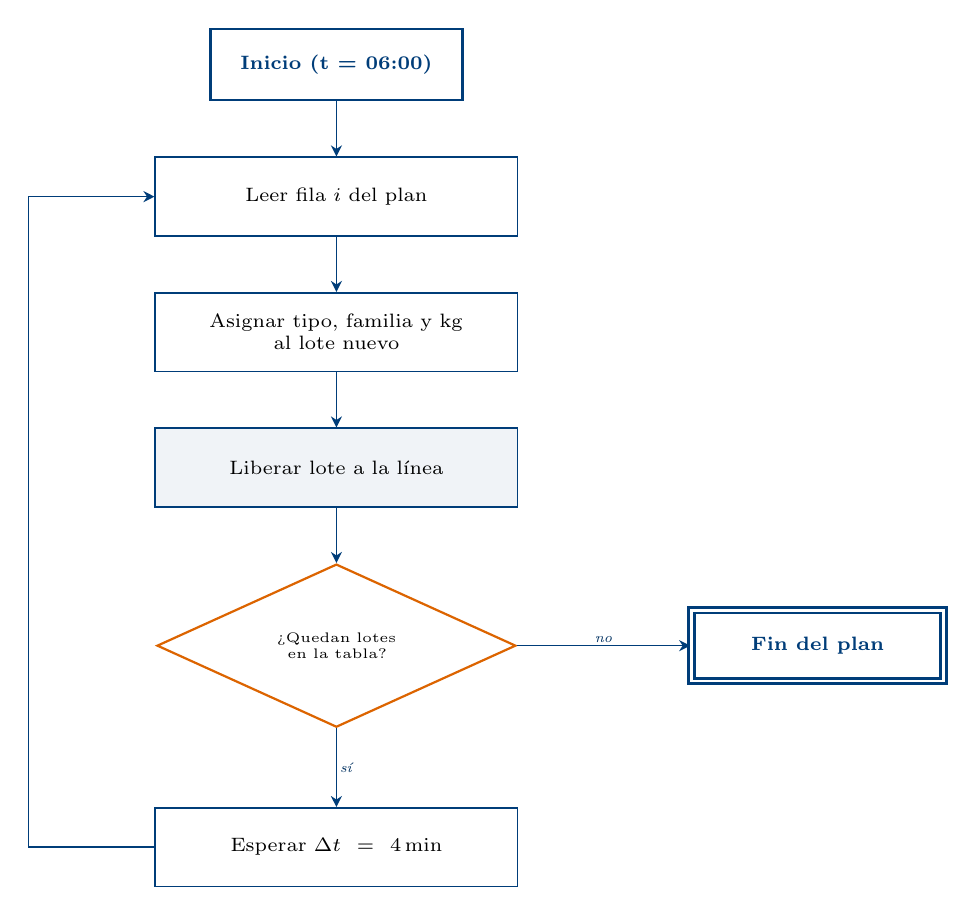
\begin{tikzpicture}[node distance=7mm and 10mm]
  \node[fc/start] (s) {Inicio (t = 06:00)};
  \node[fc/op, below=of s] (l1) {Leer fila $i$ del plan};
  \node[fc/op, below=of l1] (l2) {Asignar tipo, familia y kg\\al lote nuevo};
  \node[fc/op2, below=of l2] (l3) {Liberar lote a la l\'inea};
  \node[fc/dec, below=of l3] (d1) {¿Quedan lotes\\en la tabla?};
  \node[fc/op, below=of d1, yshift=-3mm] (l4) {Esperar $\Delta t = 4$\,min};
  \node[fc/end, right=22mm of d1] (e) {Fin del plan};

  \draw[fc/arr] (s)  -- (l1);
  \draw[fc/arr] (l1) -- (l2);
  \draw[fc/arr] (l2) -- (l3);
  \draw[fc/arr] (l3) -- (d1);
  \draw[fc/arr] (d1.south) -- node[fc/lbl, right]{s\'i} (l4.north);
  \draw[fc/arr] (l4.west) -- ++(-1.6,0) |- (l1.west);
  \draw[fc/arr] (d1.east) -- node[fc/lbl, above]{no} (e.west);
\end{tikzpicture}
\caption{Algoritmo de liberaci\'on bajo pol\'itica Plan Puro.}
\label{fig:plan_puro}
\end{figure}

\subsection{Pol\'itica H\'ibrida: Revisor de D\'eficit}

\begin{figure}[H]
\centering
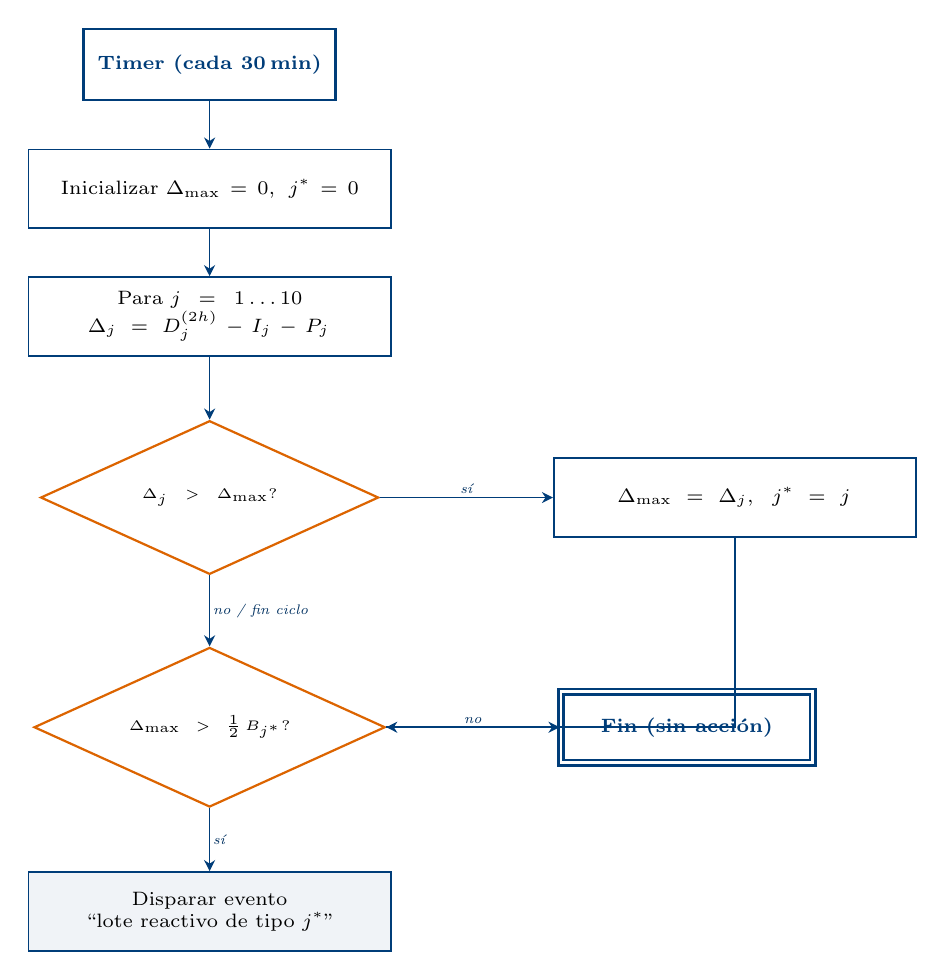
\begin{tikzpicture}[node distance=6mm and 10mm]
  \node[fc/start] (s) {Timer (cada 30\,min)};
  \node[fc/op, below=of s] (l1) {Inicializar $\Delta_{\max}=0,\;j^*=0$};
  \node[fc/op, below=of l1] (l2) {Para $j = 1\ldots10$\\
        $\Delta_j = D^{(2h)}_j - I_j - P_j$};
  \node[fc/dec, below=of l2, yshift=-2mm] (d1) {$\Delta_j > \Delta_{\max}$?};
  \node[fc/op, right=22mm of d1] (l3) {$\Delta_{\max}=\Delta_j,\;j^*=j$};
  \node[fc/dec, below=of d1, yshift=-3mm] (d2) {$\Delta_{\max}
        > \tfrac{1}{2}\,B_{j^*}$?};
  \node[fc/op2, below=of d2, yshift=-2mm] (l4) {Disparar evento\\
        ``lote reactivo de tipo $j^*$''};
  \node[fc/end, right=22mm of d2] (e) {Fin (sin acci\'on)};

  \draw[fc/arr] (s)  -- (l1);
  \draw[fc/arr] (l1) -- (l2);
  \draw[fc/arr] (l2) -- (d1);
  \draw[fc/arr] (d1.east) -- node[fc/lbl, above]{s\'i} (l3.west);
  \draw[fc/arr] (l3.south) |- (d2.east);
  \draw[fc/arr] (d1.south) -- node[fc/lbl, right]{no / fin ciclo} (d2.north);
  \draw[fc/arr] (d2.south) -- node[fc/lbl, right]{s\'i} (l4.north);
  \draw[fc/arr] (d2.east) -- node[fc/lbl, above]{no} (e.west);
\end{tikzpicture}
\caption{Algoritmo del revisor de d\'eficit bajo pol\'itica H\'ibrida.
$D^{(2h)}_j$ es la demanda esperada del SKU $j$ a 2\,h vista, $I_j$ es el
inventario en g\'ondola, $P_j$ los kg en pipeline y $B_j$ el tama\~no de lote.}
\label{fig:revisor_deficit}
\end{figure}

\subsection{Pol\'itica PULL con EOQ Estoc\'astico}

\begin{figure}[H]
\centering
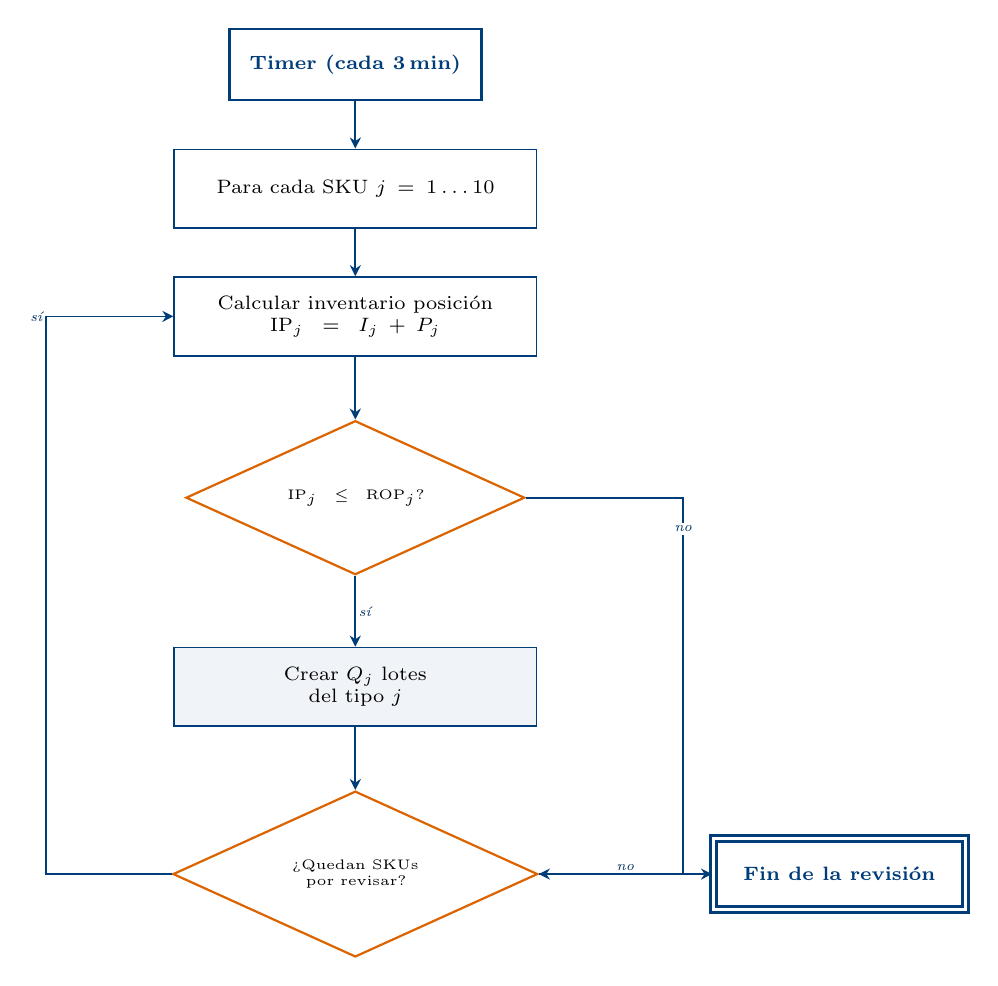
\begin{tikzpicture}[node distance=6mm and 10mm]
  \node[fc/start] (s) {Timer (cada 3\,min)};
  \node[fc/op, below=of s] (l1) {Para cada SKU $j = 1\ldots10$};
  \node[fc/op, below=of l1] (l2) {Calcular inventario posici\'on\\
        $\mathrm{IP}_j = I_j + P_j$};
  \node[fc/dec, below=of l2, yshift=-2mm] (d1) {$\mathrm{IP}_j \leq \mathrm{ROP}_j$?};
  \node[fc/op2, below=of d1, yshift=-3mm] (l3) {Crear $Q_j$ lotes\\
        del tipo $j$};
  \node[fc/dec, below=of l3, yshift=-2mm] (d2) {¿Quedan SKUs\\por revisar?};
  \node[fc/end, right=22mm of d2] (e) {Fin de la revisi\'on};

  \draw[fc/arr] (s)  -- (l1);
  \draw[fc/arr] (l1) -- (l2);
  \draw[fc/arr] (l2) -- (d1);
  \draw[fc/arr] (d1.south) -- node[fc/lbl, right]{s\'i} (l3.north);
  \draw[fc/arr] (d1.east) -- ++(2.0,0) |- (d2.east)
        node[fc/lbl, pos=0.05, above]{no};
  \draw[fc/arr] (l3.south) -- (d2.north);
  \draw[fc/arr] (d2.west) -- ++(-1.6,0) |- (l2.west)
        node[fc/lbl, midway, left]{s\'i};
  \draw[fc/arr] (d2.east) -- node[fc/lbl, above]{no} (e.west);
\end{tikzpicture}
\caption{Algoritmo de control de inventario bajo pol\'itica PULL con EOQ
estoc\'astico. $\mathrm{IP}_j$ es el inventario posici\'on; $\mathrm{ROP}_j$ y
$Q_j$ se precalculan anal\'iticamente.}
\label{fig:pull_eoq}
\end{figure}

\subsection{Llegada de Clientes (NHPP)}

\begin{figure}[H]
\centering
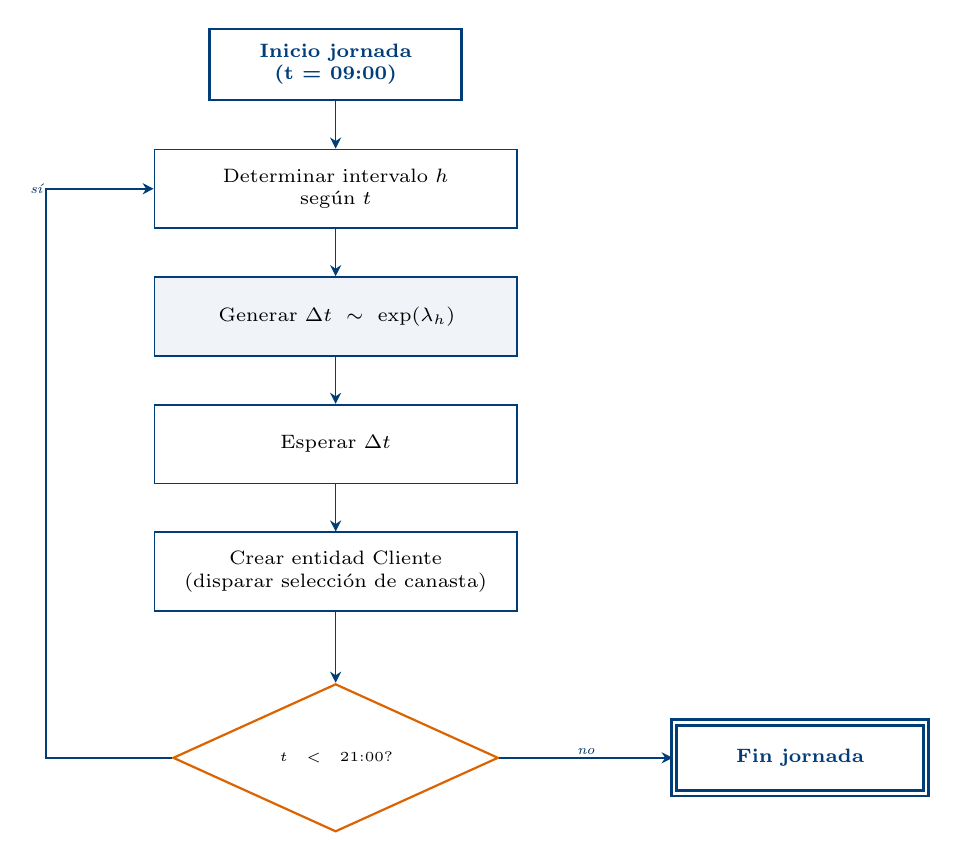
\begin{tikzpicture}[node distance=6mm and 8mm]
  \node[fc/start] (s) {Inicio jornada\\(t = 09:00)};
  \node[fc/op, below=of s] (l1) {Determinar intervalo $h$\\seg\'un $t$};
  \node[fc/op2, below=of l1] (l2) {Generar
        $\Delta t \sim \exp(\lambda_h)$};
  \node[fc/op, below=of l2] (l3) {Esperar $\Delta t$};
  \node[fc/op, below=of l3] (l4) {Crear entidad Cliente\\(disparar selecci\'on
        de canasta)};
  \node[fc/dec, below=of l4, yshift=-3mm] (d1) {$t < 21{:}00$?};
  \node[fc/end, right=22mm of d1] (e) {Fin jornada};

  \draw[fc/arr] (s)  -- (l1);
  \draw[fc/arr] (l1) -- (l2);
  \draw[fc/arr] (l2) -- (l3);
  \draw[fc/arr] (l3) -- (l4);
  \draw[fc/arr] (l4) -- (d1);
  \draw[fc/arr] (d1.west) -- ++(-1.6,0) |- (l1.west)
        node[fc/lbl, midway, left]{s\'i};
  \draw[fc/arr] (d1.east) -- node[fc/lbl, above]{no} (e.west);
\end{tikzpicture}
\caption{Generaci\'on de clientes seg\'un Proceso de Poisson No Homog\'eneo.
$\lambda_h$ se actualiza autom\'aticamente al cambiar de intervalo horario.}
\label{fig:nhpp}
\end{figure}

\subsection{Composici\'on de Canasta del Cliente}

\begin{figure}[H]
\centering
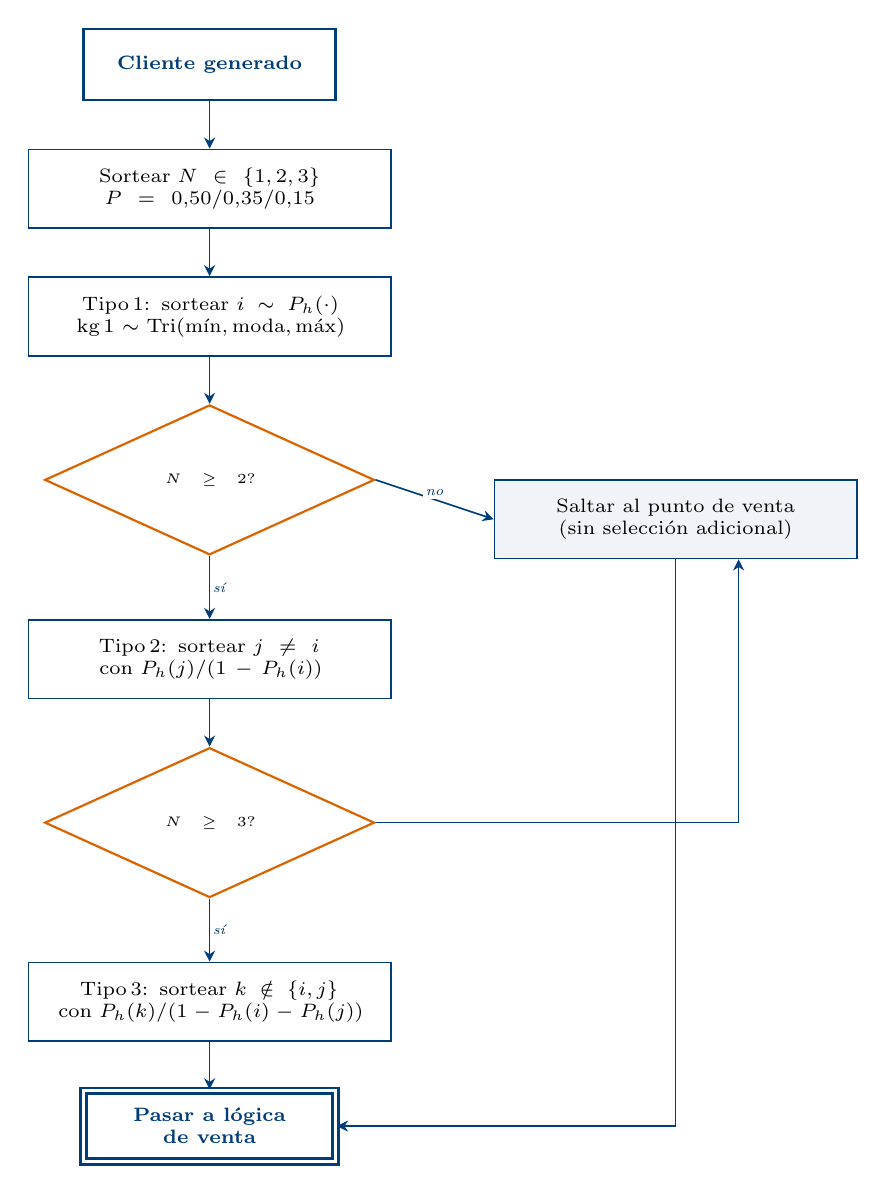
\begin{tikzpicture}[node distance=6mm and 8mm]
  \node[fc/start] (s) {Cliente generado};
  \node[fc/op, below=of s] (l1) {Sortear $N \in \{1,2,3\}$\\
        $P=0{,}50/0{,}35/0{,}15$};
  \node[fc/op, below=of l1] (l2) {Tipo\,1: sortear $i \sim P_h(\cdot)$\\
        kg\,1 $\sim$ Tri$(\text{m\'in},\text{moda},\text{m\'ax})$};
  \node[fc/dec, below=of l2] (d1) {$N \geq 2$?};
  \node[fc/op, below=of d1, yshift=-2mm] (l3) {Tipo\,2: sortear $j \neq i$\\
        con $P_h(j)/(1-P_h(i))$};
  \node[fc/dec, below=of l3] (d2) {$N \geq 3$?};
  \node[fc/op, below=of d2, yshift=-2mm] (l4) {Tipo\,3: sortear
        $k \notin \{i,j\}$\\con $P_h(k)/(1-P_h(i)-P_h(j))$};
  \node[fc/end, below=of l4] (e) {Pasar a l\'ogica\\de venta};
  \node[fc/op2, right=15mm of d1, yshift=-5mm] (skip) {Saltar al punto de
        venta\\(sin selecci\'on adicional)};

  \draw[fc/arr] (s)  -- (l1);
  \draw[fc/arr] (l1) -- (l2);
  \draw[fc/arr] (l2) -- (d1);
  \draw[fc/arr] (d1.south) -- node[fc/lbl, right]{s\'i} (l3.north);
  \draw[fc/arr] (l3.south) -- (d2.north);
  \draw[fc/arr] (d2.south) -- node[fc/lbl, right]{s\'i} (l4.north);
  \draw[fc/arr] (l4.south) -- (e.north);
  \draw[fc/arr] (d1.east) -- node[fc/lbl, above]{no} (skip.west);
  \draw[fc/arr] (d2.east) -| ([xshift=8mm]skip.south);
  \draw[fc/arr] (skip.south) |- (e.east);
\end{tikzpicture}
\caption{Algoritmo de composici\'on de canasta del cliente. $P_h(\cdot)$ es
la distribuci\'on marginal horaria; los sorteos del 2\textsuperscript{o} y
3\textsuperscript{er} tipo usan probabilidades condicionales sin reemplazo.}
\label{fig:canasta}
\end{figure}

\subsection{L\'ogica de Venta Todo-o-Nada}

\begin{figure}[H]
\centering
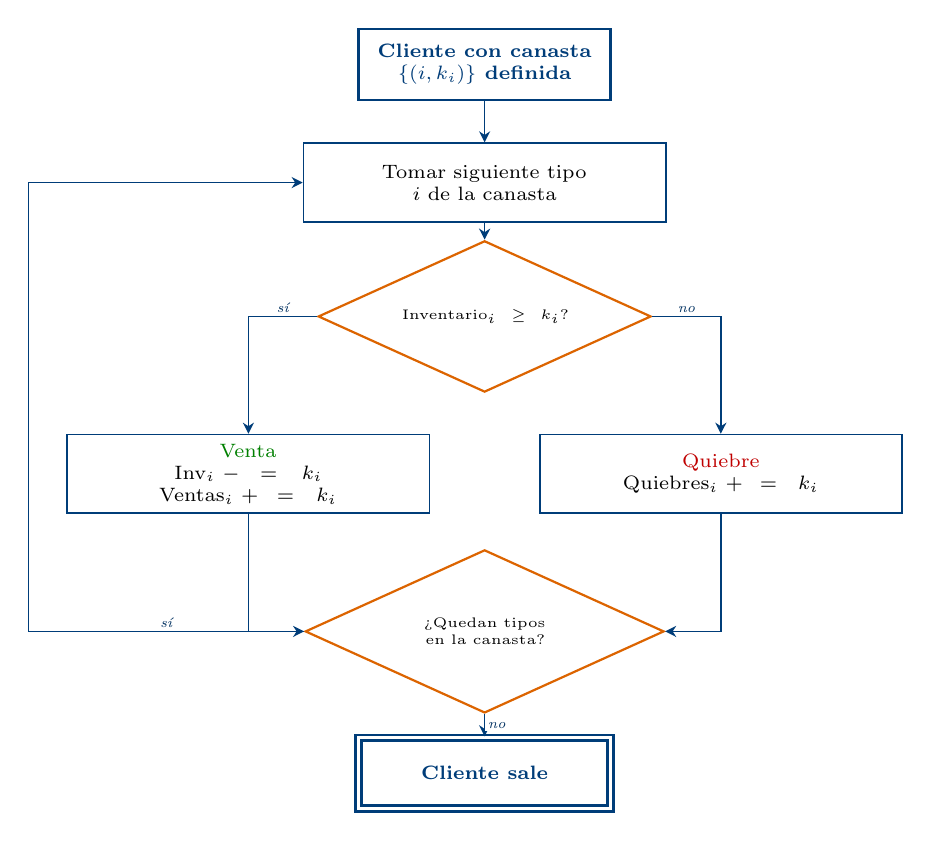
\begin{tikzpicture}[x=1cm, y=1cm]
  \node[fc/start] at (6, 9.5) (s) {Cliente con canasta\\$\{(i, k_i)\}$ definida};
  \node[fc/op]    at (6, 8.0) (l1) {Tomar siguiente tipo\\$i$ de la canasta};
  \node[fc/dec]   at (6, 6.3) (d1) {Inventario$_i \geq k_i$?};
  \node[fc/op]    at (3, 4.3) (l2)
        {{\color{verdeOK}Venta}\\Inv$_i$ $-=\,k_i$\\Ventas$_i$ $+=\,k_i$};
  \node[fc/op]    at (9, 4.3) (l3)
        {{\color{rojoAlerta}Quiebre}\\Quiebres$_i$ $+=\,k_i$};
  \node[fc/dec]   at (6, 2.3) (d2) {¿Quedan tipos\\en la canasta?};
  \node[fc/end]   at (6, 0.5) (e)  {Cliente sale};

  \draw[fc/arr] (s)  -- (l1);
  \draw[fc/arr] (l1) -- (d1);
  \draw[fc/arr] (d1.west) -| node[fc/lbl, above, pos=0.25]{s\'i} (l2.north);
  \draw[fc/arr] (d1.east) -| node[fc/lbl, above, pos=0.25]{no} (l3.north);
  \draw[fc/arr] (l2.south) |- (d2.west);
  \draw[fc/arr] (l3.south) |- (d2.east);
  % Loop "sí" — ruteado fuera del área de Venta (izquierda)
  \draw[fc/arr] (d2.west) -- ++(-3.5,0)
        node[fc/lbl, midway, above]{s\'i}
        |- (l1.west);
  \draw[fc/arr] (d2.south) -- node[fc/lbl, right]{no} (e.north);
\end{tikzpicture}
\caption{L\'ogica de venta todo-o-nada. Cada tipo de pan en la canasta se
procesa independientemente; un quiebre en un tipo no impide la venta de los
restantes.}
\label{fig:venta}
\end{figure}

\subsection{Pol\'itica de Carga del Horno}

\begin{figure}[H]
\centering
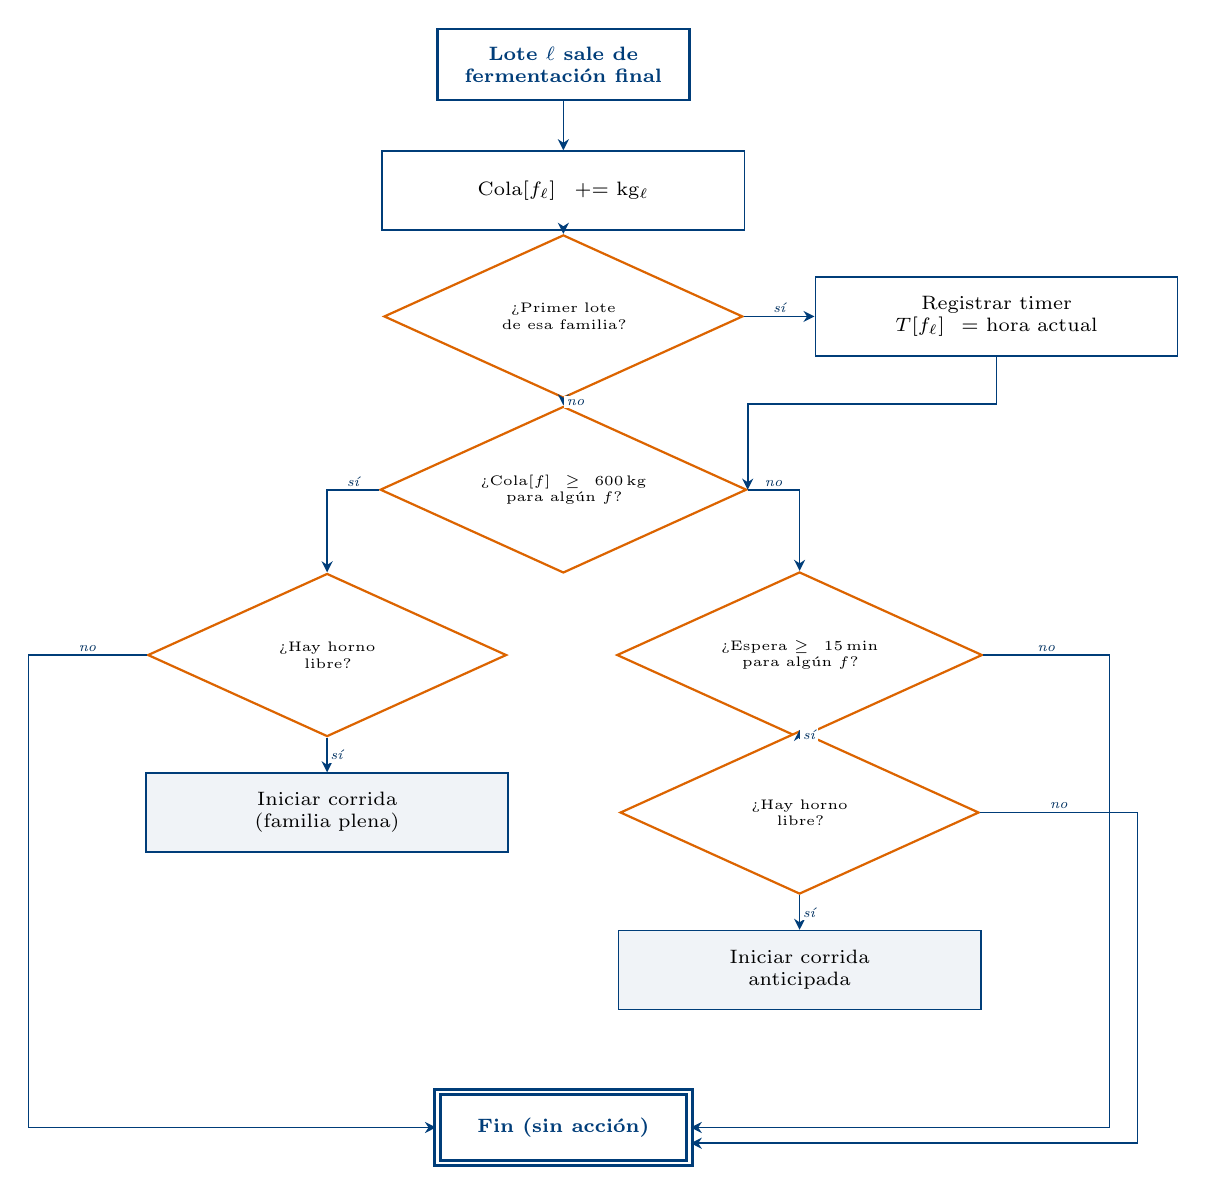
\begin{tikzpicture}[x=1cm, y=1cm]
  % Cabecera: ingreso y registro de timer
  \node[fc/start] at (5, 13.0)  (s)  {Lote $\ell$ sale de\\fermentaci\'on final};
  \node[fc/op]    at (5, 11.4)  (l1) {Cola$[f_\ell]\mathrel{+}= $ kg$_\ell$};
  \node[fc/dec]   at (5,  9.8)  (d1) {¿Primer lote\\de esa familia?};
  \node[fc/op]    at (10.5, 9.8)(l2) {Registrar timer\\
        $T[f_\ell] = $ hora actual};

  % Decisión principal de capacidad
  \node[fc/dec]   at (5,  7.6)  (d2) {¿Cola$[f] \geq 600$\,kg\\
        para alg\'un $f$?};

  % Rama izquierda (sí, carga plena): d3 + acción
  \node[fc/dec]   at (2,  5.5)  (d3) {¿Hay horno\\libre?};
  \node[fc/op2]   at (2,  3.5)  (l3) {Iniciar corrida\\(familia plena)};

  % Rama derecha (no, evaluar espera ≥ 15 min): d4 → d5 + acción
  \node[fc/dec]   at (8,  5.5)  (d4) {¿Espera $\geq 15$\,min\\
        para alg\'un $f$?};
  \node[fc/dec]   at (8,  3.5)  (d5) {¿Hay horno\\libre?};
  \node[fc/op2]   at (8,  1.5)  (l4) {Iniciar corrida\\anticipada};

  % Punto común de salida (Fin) abajo en el centro
  \node[fc/end]   at (5, -0.5)  (e)  {Fin (sin acci\'on)};

  % --- Flujo principal ---
  \draw[fc/arr] (s)  -- (l1);
  \draw[fc/arr] (l1) -- (d1);
  \draw[fc/arr] (d1.east) -- node[fc/lbl, above]{s\'i} (l2.west);
  \draw[fc/arr] (l2.south) -- ++(0,-0.6) -| (d2.east);
  \draw[fc/arr] (d1.south) -- node[fc/lbl, right]{no} (d2.north);

  % Bifurcación de d2
  \draw[fc/arr] (d2.west) -| node[fc/lbl, above, pos=0.25]{s\'i} (d3.north);
  \draw[fc/arr] (d2.east) -| node[fc/lbl, above, pos=0.25]{no} (d4.north);

  % Acciones "sí"
  \draw[fc/arr] (d3.south) -- node[fc/lbl, right]{s\'i} (l3.north);
  \draw[fc/arr] (d4.south) -- node[fc/lbl, right]{s\'i} (d5.north);
  \draw[fc/arr] (d5.south) -- node[fc/lbl, right]{s\'i} (l4.north);

  % --- Rutas "no" hacia Fin (todas convergen abajo, sin atravesar cajas) ---
  % d3.no: sale por el oeste, baja por el extremo izquierdo y entra a Fin por su oeste
  \draw[fc/arr] (d3.west) -- ++(-1.5,0)
        node[fc/lbl, midway, above]{no}
        |- (e.west);
  % d4.no: sale por el este, baja por el extremo derecho y entra a Fin por su este
  \draw[fc/arr] (d4.east) -- ++(1.6,0)
        node[fc/lbl, midway, above]{no}
        |- (e.east);
  % d5.no: sale por el este, baja y se une al mismo borde derecho hasta Fin
  \draw[fc/arr] (d5.east) -- ++(2.0,0)
        node[fc/lbl, midway, above]{no}
        |- ([yshift=-2mm]e.east);
\end{tikzpicture}
\caption{Algoritmo de pol\'itica de carga del horno. La evaluaci\'on
considera las tres familias simult\'aneamente para que una familia ya llena no
quede bloqueada esperando un lote de otra familia.}
\label{fig:carga_horno}
\end{figure}

\newpage

% ============================================================
%  ANEXO B — Matriz Maestra de Escenarios
% ============================================================
\section{Matriz Maestra de Escenarios}
\label{app:escenarios}

% TODO: redactar en conjunto

\newpage

% ============================================================
%  ANEXO C — Tablas de Resultados Detallados
% ============================================================
\section{Tablas de Resultados Detallados}
\label{app:resultados}

% TODO: redactar en conjunto

\end{document}
